\documentclass[12pt, oneside]{article}   	% use "amsart" instead of "article" for AMSLaTeX format
\usepackage{geometry}                		% See geometry.pdf to learn the layout options. There are lots.
\geometry{a4paper, total={6.8in, 8.5in}}
\usepackage{fancyhdr}
\usepackage{amsmath}
\usepackage{amssymb}
\usepackage{graphicx}				% Use pdf, png, jpg, or eps§ with pdflatex; use eps in DVI mode
\graphicspath{ {./} }
\usepackage{enumitem}
\usepackage{float}


\begin{document}
\pagestyle{fancy}
\fancyhead{}
\fancyhead[LO]{\textbf{CSE 5370}\\\textbf{BIO INFORMATICS}}
\fancyhead[RO]{\textbf{Sanjana Reddy Thigulla}\\1002142811}
\fancyhead[CO]{\LARGE{\textbf{Homework-3}}}



\begin{enumerate}
\item \textbf{Substitution Matrices}\\
\\
\begin{tabular}{|c|c|c|c|c|}
\hline
   & A & G & T & C \\
\hline
A & 1 & -4 & -1 & -1 \\
G & -4 & 1 & -1 & -1  \\
T & -1 & -1 & 1 & -4  \\
G & -1 & -1 & -4 & 1  \\
\hline
\end{tabular}\\
\\
 Given that the transition mutations (A $\leftrightarrow$ G and T $\leftrightarrow$ C) are less common than tranversions (A $\leftrightarrow$ T, A $\leftrightarrow$ C, G $\leftrightarrow$ T, and G $\leftrightarrow$C). In the initial matrix all the mismatches are given a score of '-1'. But since a few transition mutations are less likely than the others the mismatch score should be less comparatively. So -4  has been used as the mismatch score for the less likely mutations. 
\item 
\textbf{ Global Alignment }\\
\\
Needleman-Wunsch algorithm has been used for global alignment. The code takes in 2 input sequences, substitution matrix and gap penalty. It returns alignments. 
\\
An example of sequences "gata","ctac" with gap penalty -2 and match and mismatch of 1 and -1 is given. When the function is run with this input the output obtained is depicted below.\\ 

\begin{figure}[H]
    \centering
    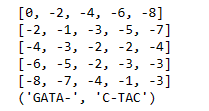
\includegraphics[width=0.3\textwidth]{globalegop}
    \caption{\footnotesize{output of the given example input sequences}}
    \label{fig:mesh1}
\end{figure}




\item 
\textbf{ Local Alignment }\\
\\
Smith-Waterman algorithm has been used for local alignment. The code takes in 2 input sequences, substitution matrix and gap penalty. It returns alignment tuples.\\
An example of sequences "gata","ctac" with gap penalty -2 and match and mismatch of 1 and -1 is given. When the function is run with this input the output obtained is depicted below.\\ 

\newpage
\begin{figure}[H]
    \centering
    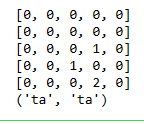
\includegraphics[width=0.2\textwidth]{localegop}
    \caption{\footnotesize{output of the given example input sequences}}
    \label{fig:mesh1}
\end{figure}

\item 
\textbf{ Custom Alignment }
\begin{itemize}
\item Using my first and last name a substitution matrix for alphabets has been created where matches are given a score of 2, semi-matches (characters in first and last name) are given a score of 1 and mismatches are given -1 . The output matrix has been pretty printed and is provided in the file "10012142811S.txt"
\item after running the custom substitution matrix with “local alignment” function , a gap penalty of -2, my concatenated name ( “sanjanareddy”) as the first string, and the pangram “thequickbrownfoxjumpsoverthelazydog” as the second string the output tuples are: \\
{[('sa', 'er'),  ('sa', 'yd'),  ('an', 'er'), ('an', 'yd'), ('nj', 'er'), ('nj', 'yd'), ('ja', 'er'), ('ja', 'yd'), ('an', 'er'), ('an', 'yd'),  ('na', 'er'), ('na', 'yd'), ('ar', 'er'), ('ar', 'yd'), ('re', 'er'), ('re', 'yd'), ('ed', 'er'), ('ed', 'yd'), ('dd', 'er'), ('dd', 'yd'), ('dy', 'er'), ('dy', 'yd')]}\\
matrix D for the input strings has been provided in the file "1002142811D.txt"




\end{itemize}
\item
\textbf{ Difficulty Adjustment }
It took me 11 -15 hours for this assignment. The first three parts took less time compared to the fourth part. I could obtain the subsitution matrix but then pretty printing was a bit confusing. I had to refer about pretty printing and also about how to give double arrows,tables  in latex . 




\end{enumerate}
\end{document}